\section{Estimating with Sums}
If we know how something changes, we can use sums to estimate, or sometimes even know exactly the net change.

\begin{example}
	A train moves at 80 miles per hour for 3 hours.
	How far does it travel?
\end{example}
\begin{answer}
	This is the kind of simple problem you might see in a physics class.
	\begin{equation*}
		\frac{80\text{mi}}{\text{hr}} \hspace{3pt} 3\text{hr} = 80\cdot 3\text{mi} = 240 \text{mi}.
	\end{equation*}
	However, if we take a look at a graph of this situation, with speed in miles per hour on the $y$ axis and time in hours on the $x$ axis, we see that the area underneath the curve from $x=0\text{hr}$ to $x=3\text{hr}$ is exactly our answer of 240 miles.
	This is not a coincidence, as what we effectively did mathematically is find the area of this rectangle.
	
	\begin{figure}[H]
		\label{constant_graph}
		\centering
		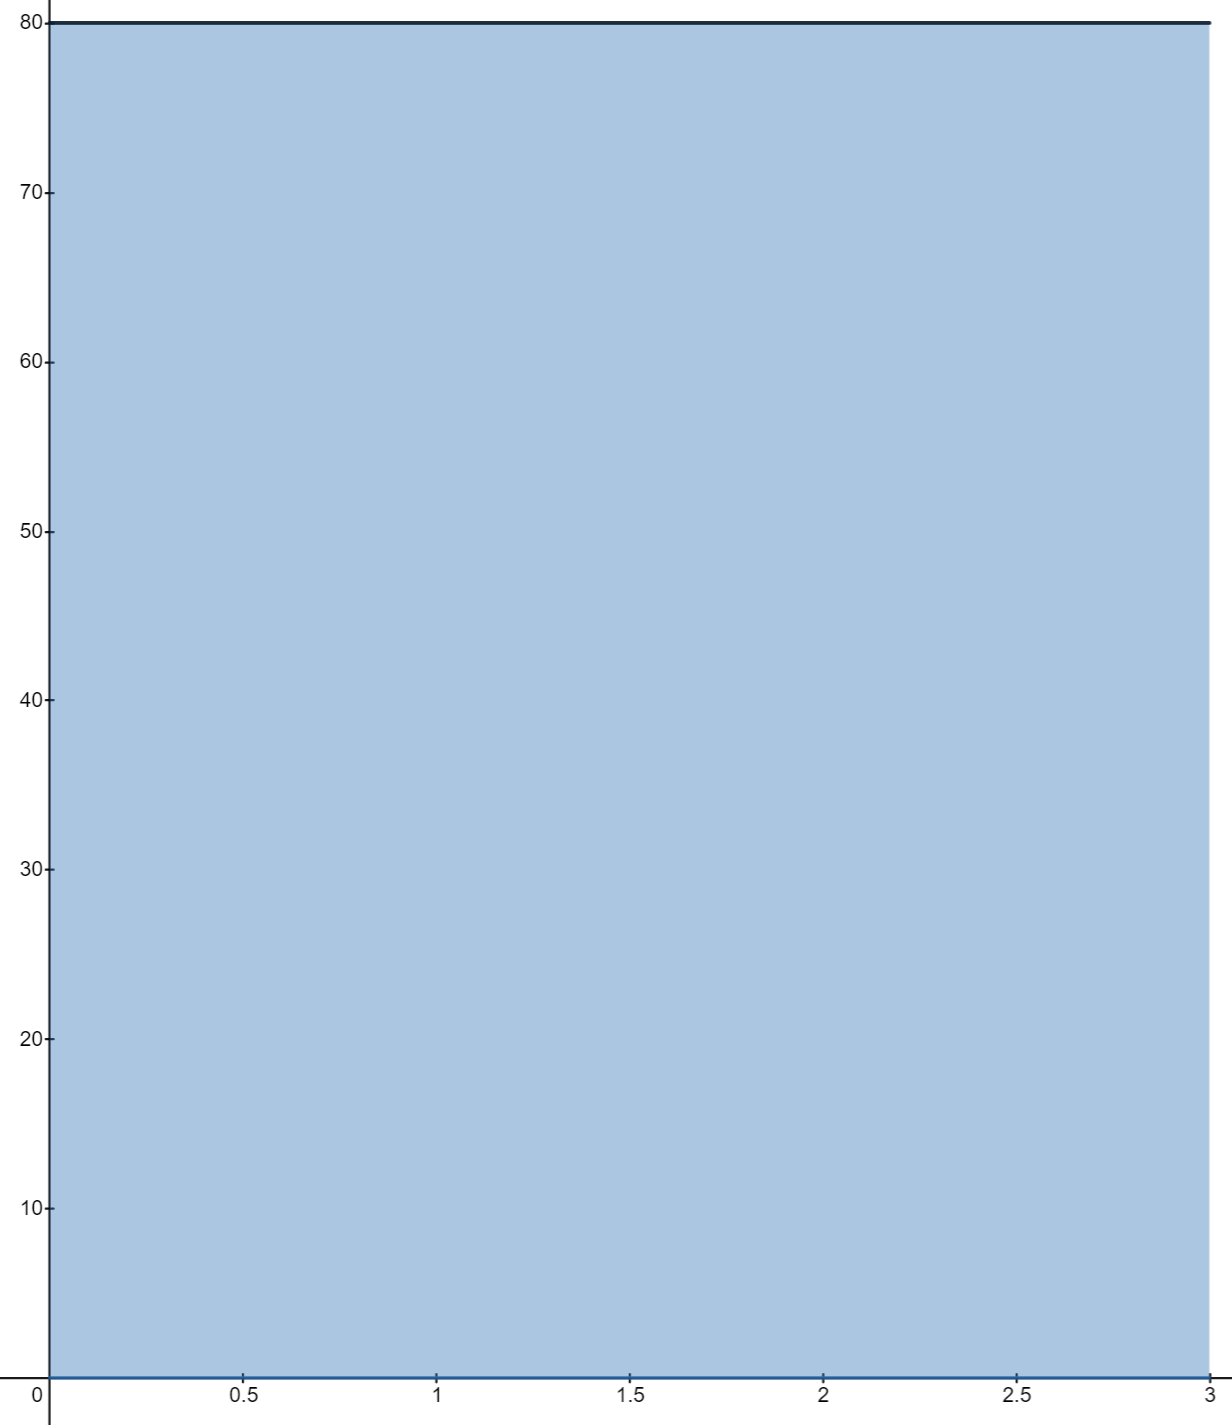
\includegraphics[width = 0.33\textwidth]{./integrals/constant_graph.png}
		\caption{\hyperref{}{}{}{Our answer is the area under the curve.}}
	\end{figure}
	\end{answer}

The same idea of finding the area under the curve works not just for constant speeds.
\begin{example}
	A particle moves at velocity $v(t) = 3t + 3$ meters per second for time $t \geq 0$.
	What is the position of the particle at $t = 2$ seconds?
\end{example}
\begin{answer}
	\begin{figure}[H]
		\label{linear_graph}
		\centering
		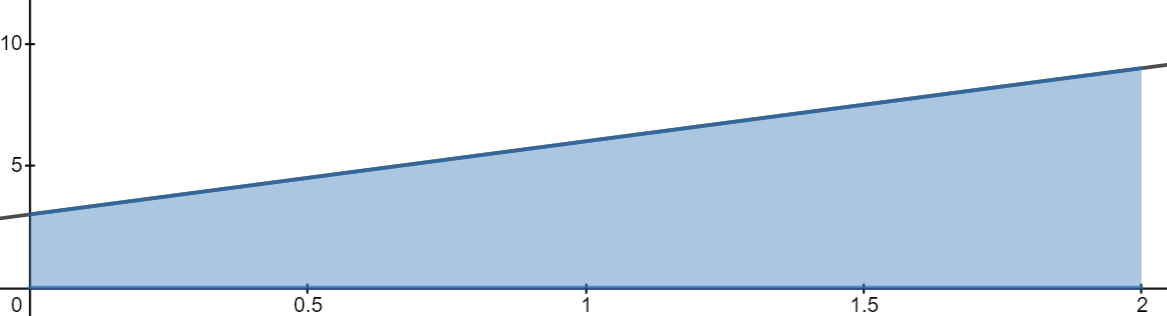
\includegraphics[width = 0.5\textwidth]{./integrals/linear_graph.png}
		\caption{\hyperref{}{}{}{Our answer is still the area under the curve.}}
	\end{figure}
	\begin{align*}
		A &= \frac{1}{2}h(b_1 + b_2) \\
		&= \frac{1}{2}(2\text{s}-0\text{s})(v(0) + v(2)) \\
		&= \frac{1}{2}(2\text{s})(3\text{m/s} + 9\text{m/s}) \\
		&= 12\text{m}.
	\end{align*}
\end{answer}

\subsubsection{Left Endpoint Approximation}
In fact, the area under the curve even works for more complicated, non-linear curves like $v(t) = t^2 + 1$.
We just need a way to find the area underneath these curves.
One idea that was used to find areas as far back as Archimedes was to estimate the complex shape using easier shapes like rectangles.
The narrower the width of each rectangle, the better the estimate becomes.
 
\begin{figure}[H]
	\label{cos_blocks}
	\centering
	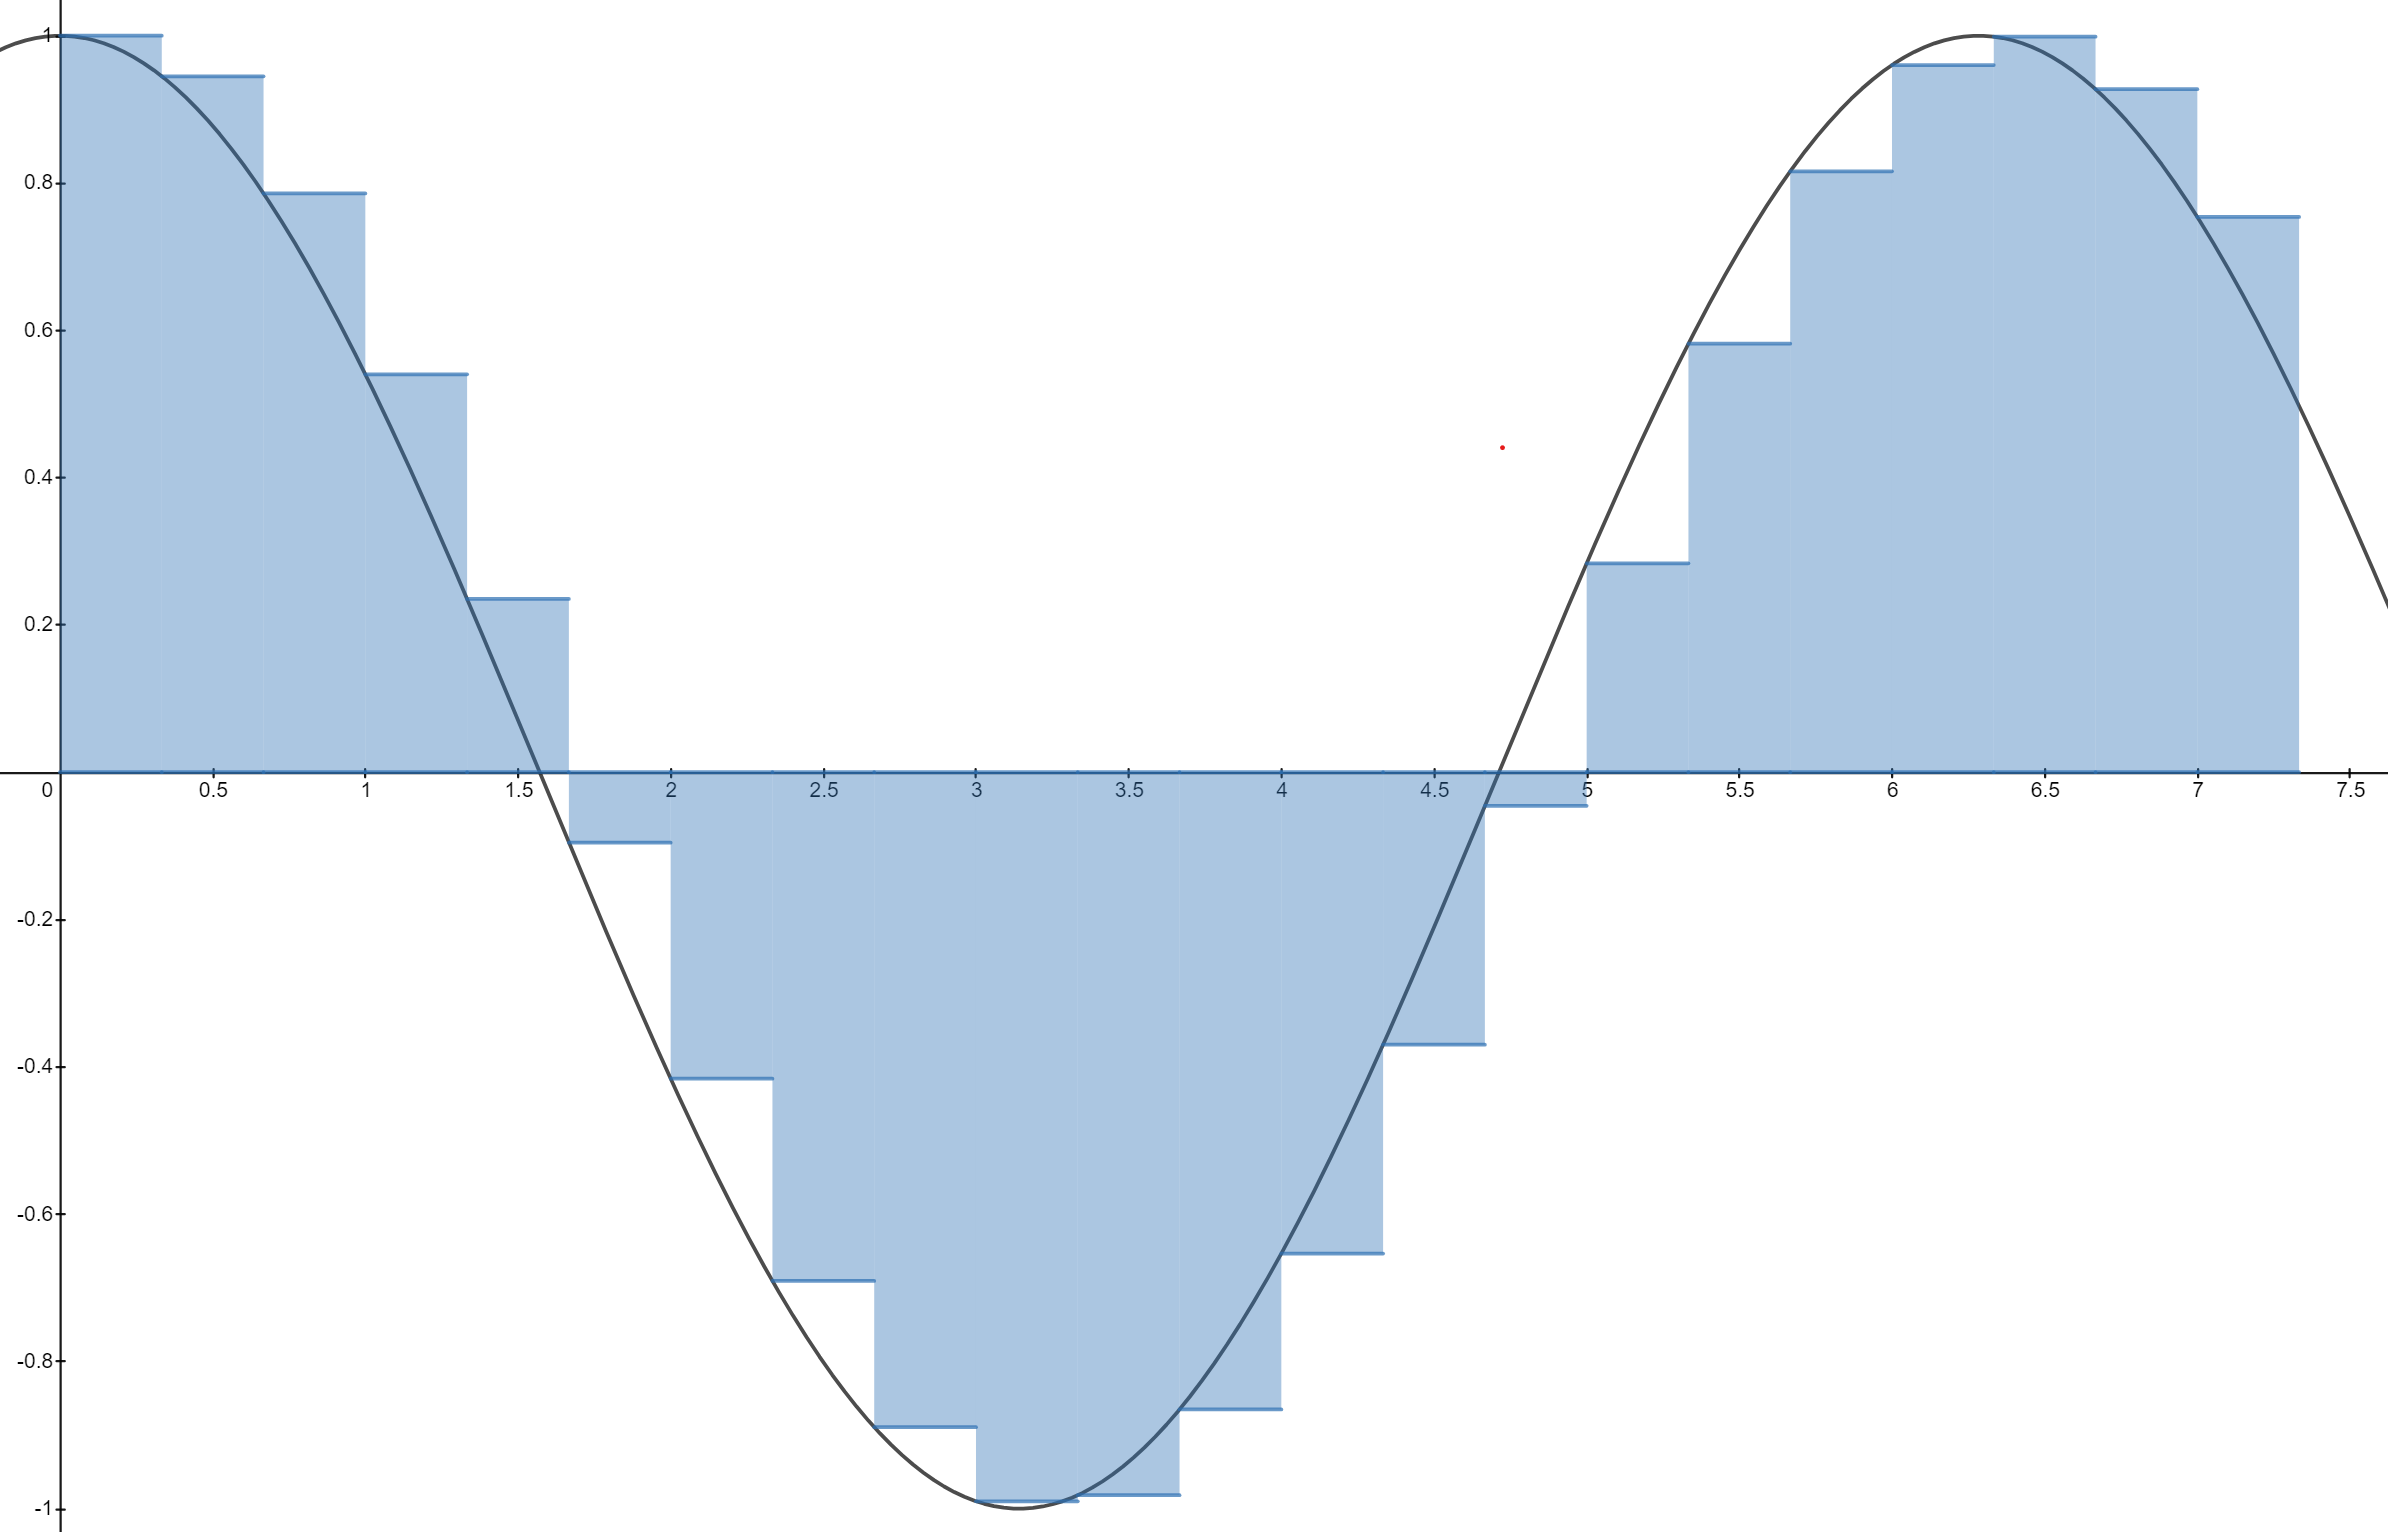
\includegraphics[width = 0.3\textwidth]{./integrals/cos_blocks1.png}
	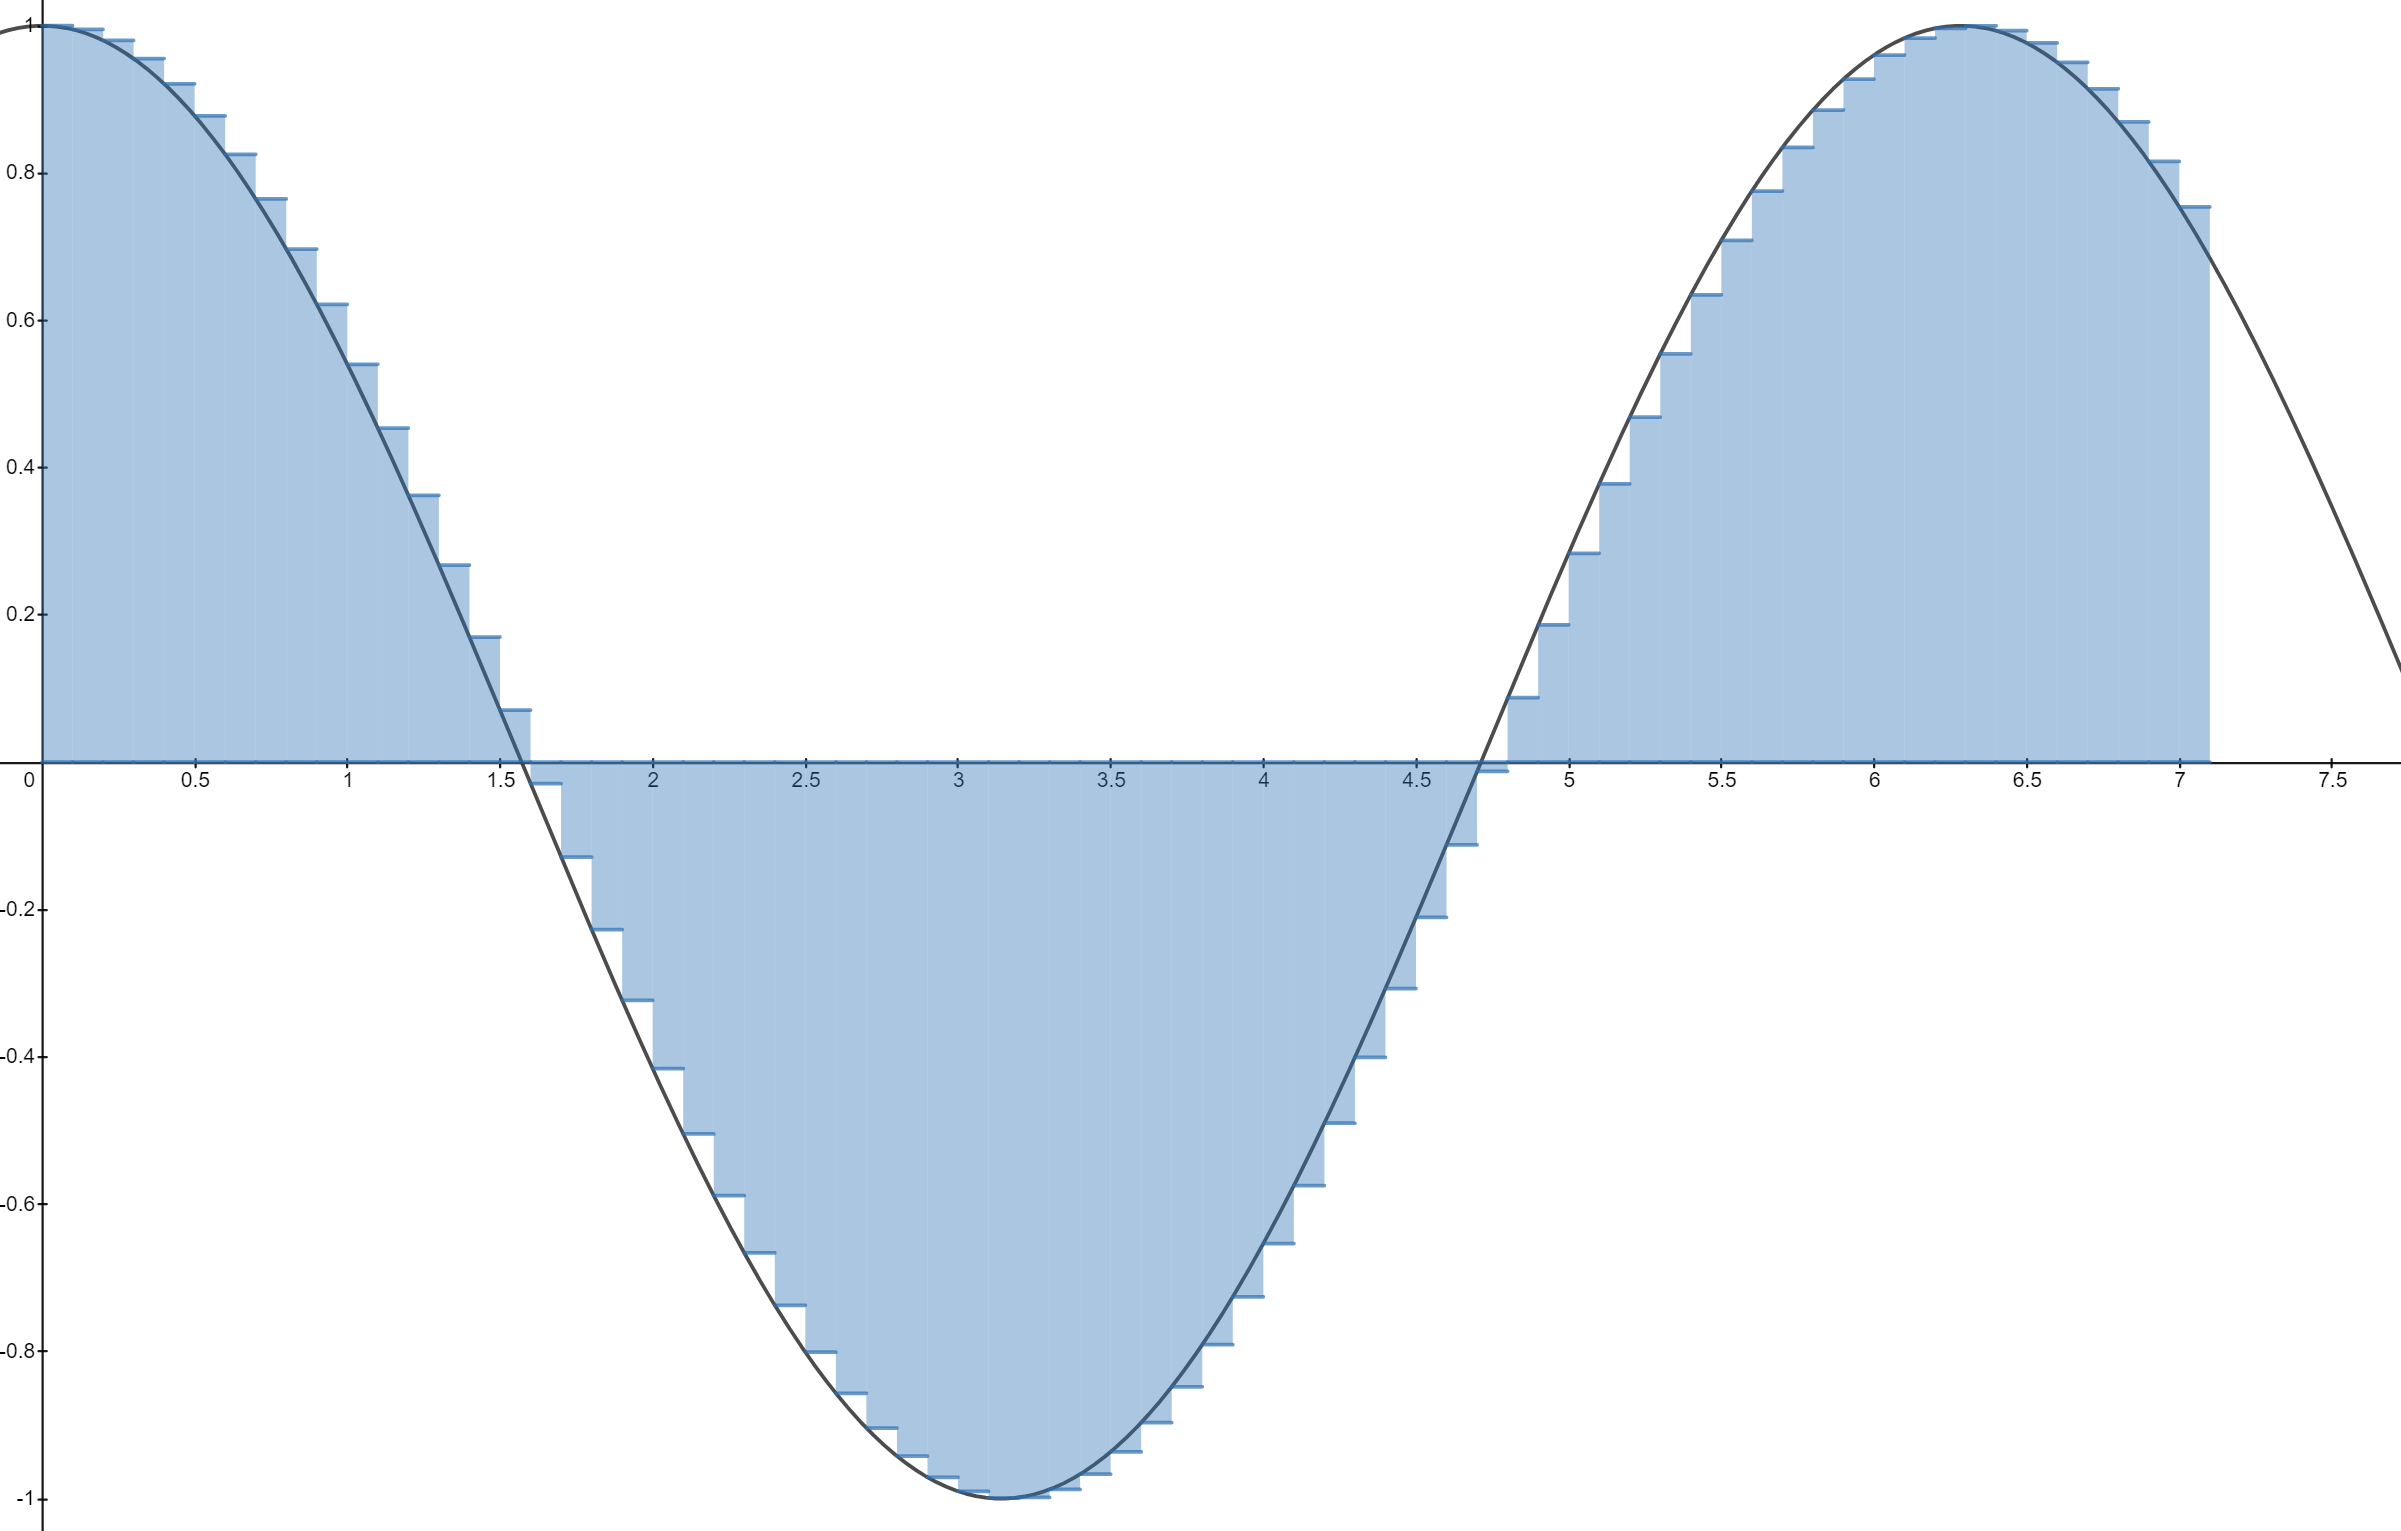
\includegraphics[width = 0.3\textwidth]{./integrals/cos_blocks2.png}
	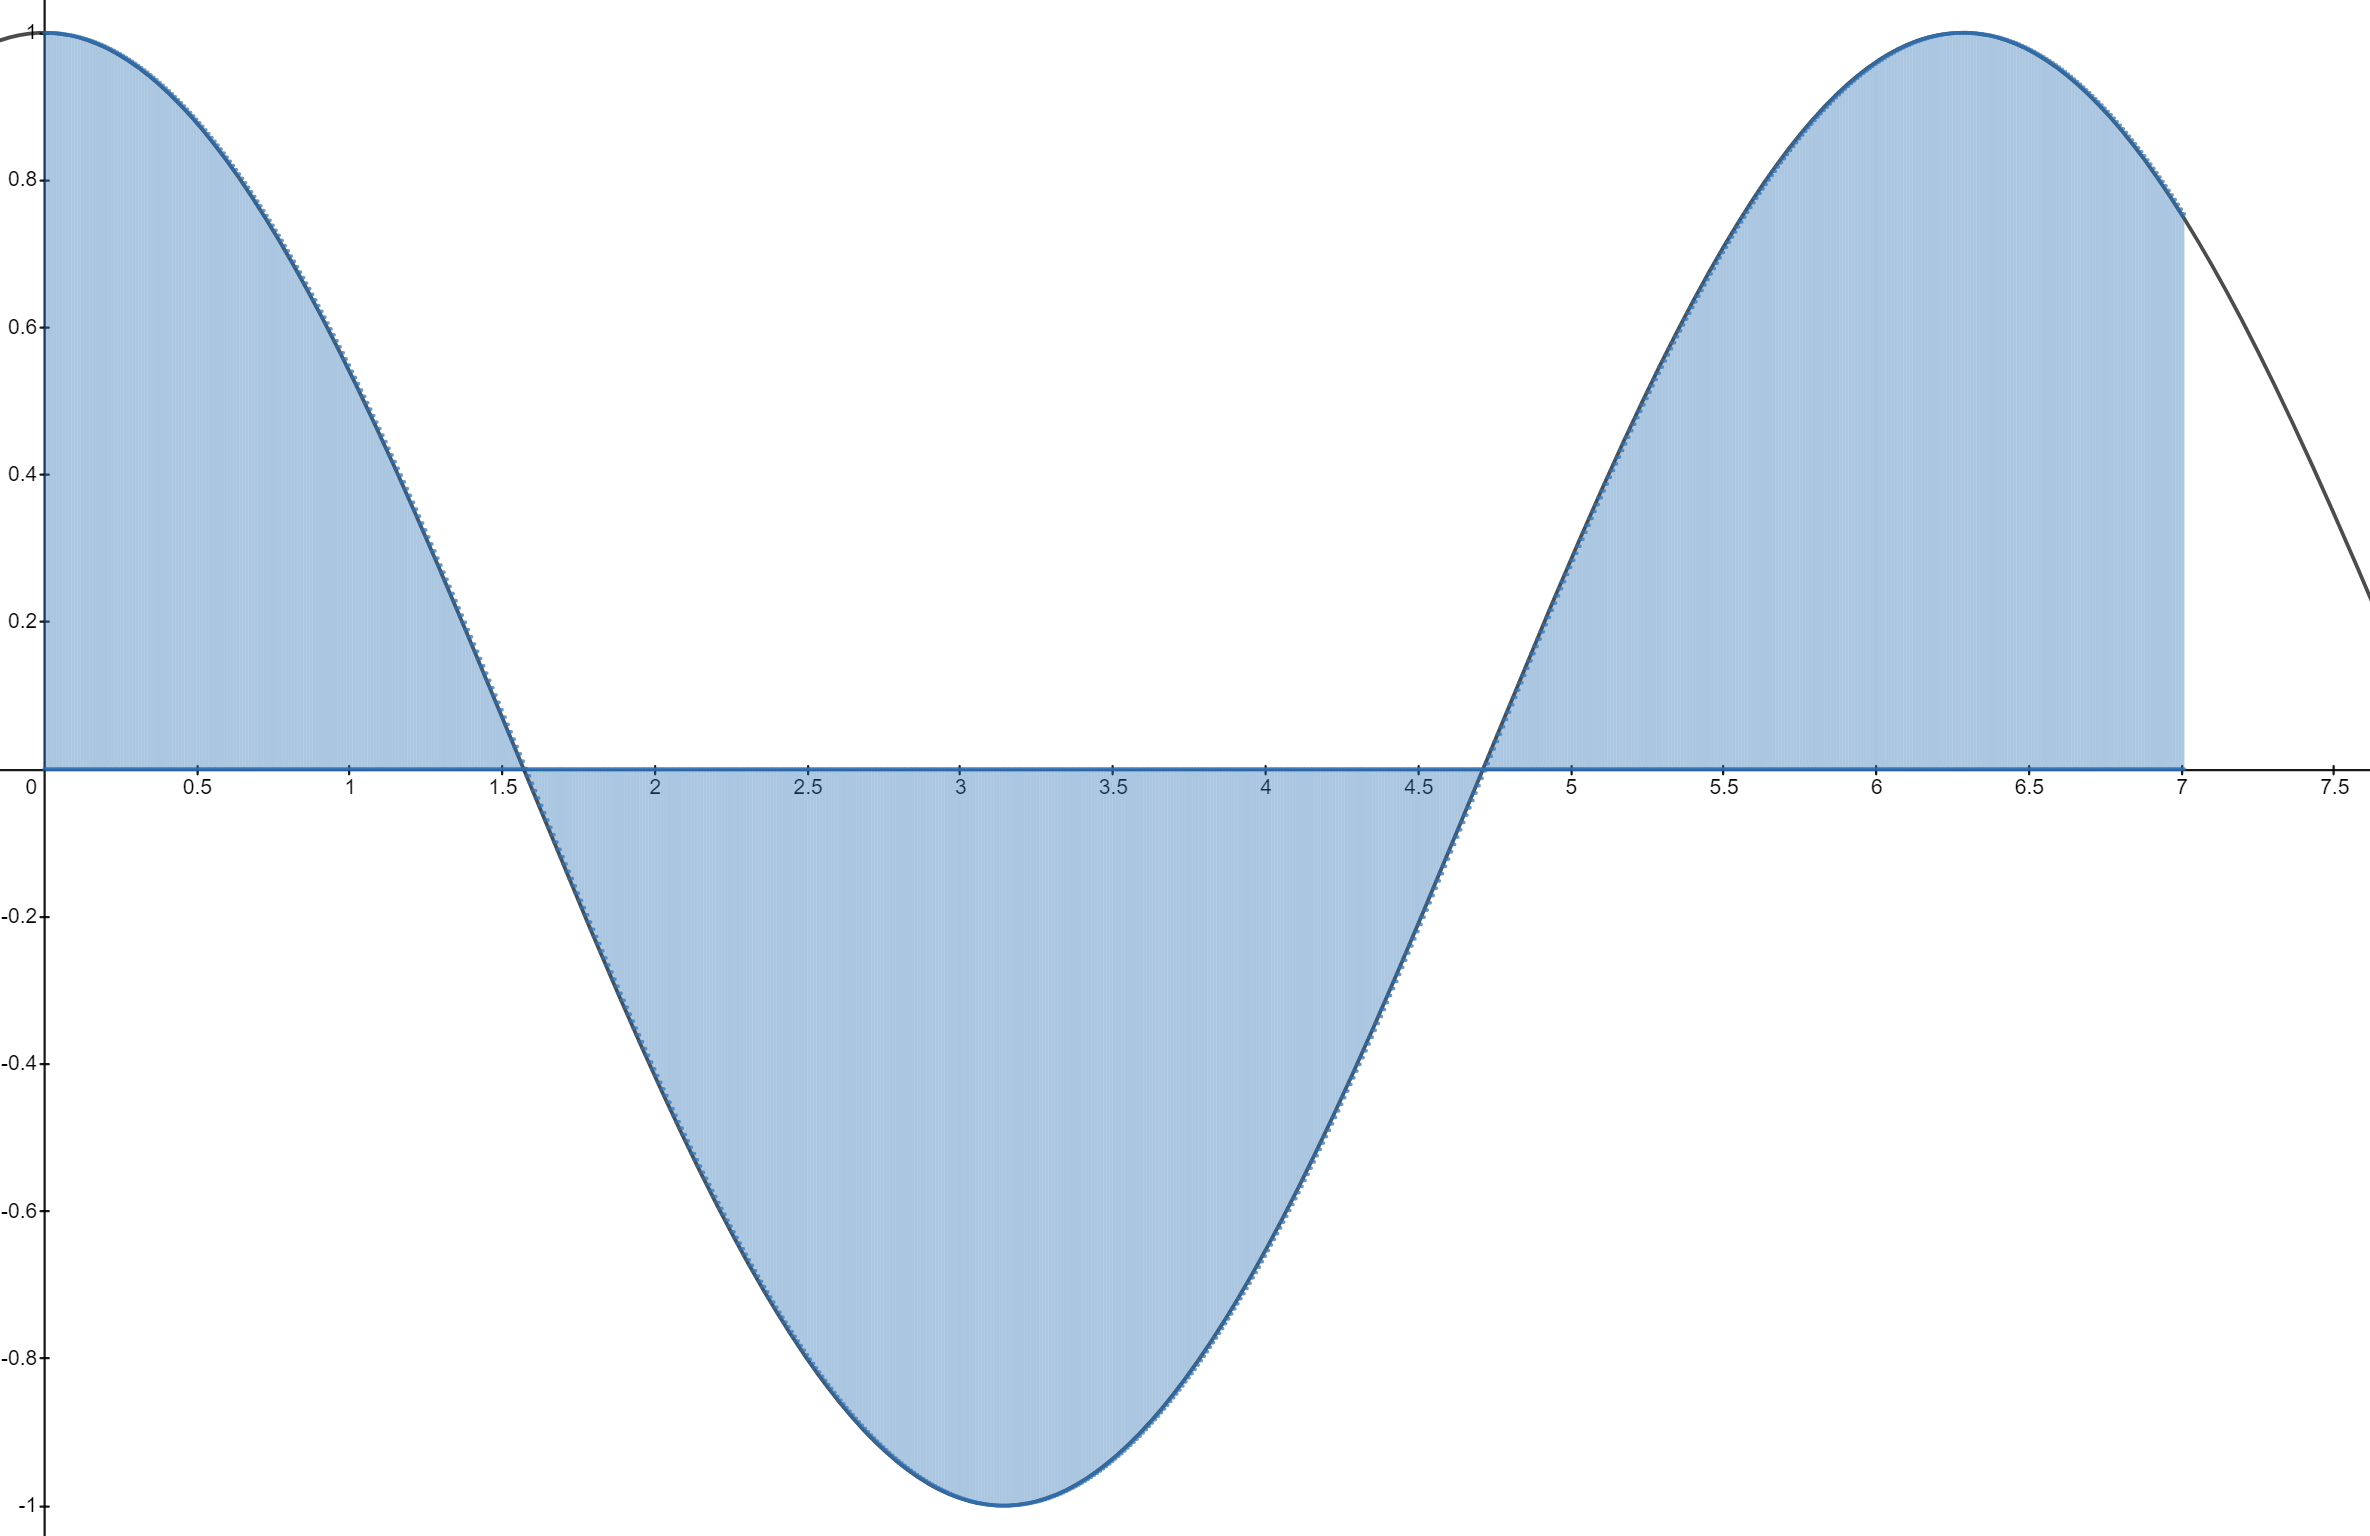
\includegraphics[width = 0.3\textwidth]{./integrals/cos_blocks3.png}
	\caption{\hyperref{}{}{}{Left Endpoint: Block widths of 1/3, 1/10, and 1/100.}}
\end{figure}


Although above we've used a left endpoint approximation, we could have also used the right endpoint or midpoint, which might give better approximations for certain types of curves.
No matter the approximation type, the estimate tends to get closer to the true area as the rectangle width is decreased.
The formulas for estimating the area of $f$ from $a$ to $b$ with $n$ rectangles are
\begin{align*}
	A_\text{left} &= \sum_{k=0}^{n-1}{f\left(a+k\Delta x\right)\Delta x} \\
	A_\text{right} &= \sum_{k=0}^{n-1}{f\left(a+(k+1)\Delta x\right)\Delta x} \\
	A_\text{mid} &= \sum_{k=0}^{n-1}{f\left(a+\frac{2k+1}{2}\Delta x\right)\Delta x} \\
	\text{where }\Delta x &= \frac{b-a}{n}.
\end{align*}

\subsubsection{Trapezoidal Rule}
Another common shape to use rather than rectangles is trapezoids.
Trapezoids allow us to find the exact area of functions made of straight lines\footnote{There are higher-order, more accurate estimations than the trapezoidal rule. The most common is Simpson's Rule. $A = \frac{2M+T}{3}$ where $M$ is the midpoint formula area and $T$ is the trapezoidal rule area. It can exactly give the area of quadratics because it corresponds to estimating areas using parabolas that intersect the curve at the left, middle, and right of each "strip".} and like the left endpoint approximation, get better the narrower the width of each trapezoid.
Starting from the formula, we can make some simplifications.
\begin{equation*}
	A = \frac{1}{2}(b_1 + b_2)h.
\end{equation*}
Now summing each of these trapezoids' areas to approximate our function $f$ from $a$ to $b$,
\begin{align*}
	A_\text{trap} &= \sum_{k=0}^{n-1}{\frac{1}{2}\left(f(a+i\Delta a) + f(a + (i+1)\Delta x)\right)\Delta x} \\
	&= \frac{\Delta x}{2}\sum_{k=0}^{n-1}{f(a + i\Delta x) + f(a + (i+1)\Delta x)} \\
	&= \frac{\Delta x}{2}\left(\left(f(a)+f(a+\Delta x)\right)+\left(f(a+\Delta x)+f(a+2\Delta x)\right)+\ldots+\left(f(a+(n-1)\Delta x)+f(a+n\Delta x)\right)\right) \\
	&= \frac{\Delta x}{2}\left(f(a) + 2f(a+\Delta x) + 2f(a + 2\Delta x) + \ldots + 2f(a+(n-1)\Delta x) + f(a+n\Delta x)\right) \\
	&= \frac{A_\text{left} + A_\text{right}}{2}.
\end{align*}

The trapezoidal rule overestimates areas when the curve is concave up and underestimates when the curve is concave down.